\documentclass[12pt]{article}
\usepackage[T2A]{fontenc}                           % пакет для підтримки кирилічних шрифтів
\usepackage[utf8]{inputenc}
\usepackage[russian,ukrainian]{babel}

\usepackage{type1ec}
\usepackage{graphicx} % Required for inserting image
\usepackage{cmap}                                   % для кодування шрифтів у pdf
\usepackage{listings, listings-rust}
\usepackage{xcolor}
\usepackage{amsmath}
\usepackage{amssymb}
\usepackage{amsfonts}
\usepackage{float}

\definecolor{codegreen}{rgb}{0,0.6,0}
\definecolor{codegray}{rgb}{0.5,0.5,0.5}
\definecolor{codepurple}{rgb}{0.58,0,0.82}
\definecolor{backcolour}{rgb}{0.95,0.95,0.92}

\usepackage{geometry}
\geometry{
    a4paper,
    left = 20mm,
    top = 20mm,
    right = 10mm,
    bottom = 20mm
}

\lstdefinestyle{mystyle}{
    backgroundcolor=\color{backcolour},   
    commentstyle=\color{codegreen},
    keywordstyle=\color{magenta},
    numberstyle=\tiny\color{codegray},
    stringstyle=\color{codepurple},
    basicstyle=\ttfamily\footnotesize,
    breakatwhitespace=false,         
    breaklines=true,                 
    captionpos=b,                    
    keepspaces=true,                 
    numbers=left,                    
    numbersep=5pt,                  
    showspaces=false,                
    showstringspaces=false,
    showtabs=false,                  
    tabsize=2
}

\lstset{style=mystyle}

\begin{document}

\include{titlepage}

\section{Опис роботи}

У даному комп'ютерному практикумі необхідно було провести атаку випадкового пошуку праобразу, та пошуку колізії, на усічену версію геш-функції, згідно мого варіанту- \emph{SHA3}. Було виконано ускладнену версію завдання, а для реалізації використовувався Rust.

За геш-функцію було взято SHA-3-224, оскільки із згенерованого геша, нам потрібно лише 4-8 останніх байтів\footnote{Також можна припустити, що цей варіант все ж трохи швидший, оскільки більший параметр $r$, проте, практика показала, що різниця між часом виконання у середньому між різними варіантами SHA-3 в реалізації rust-crypto відрізняється несуттєво.}. 224 біта $=$ 28 байтів буде генерувати наша геш функція. Масив байтів, який повертає наша геш функція, ми будемо представляти як шістнадцятковий рядок, де 1 символ-- це пів байта.

\subsection{Підхід до організації атак}

У моїй роботі, я вирішив трохи узагальнити варіанти запропонованих атак, що можливо, було не дуже вдалим рішенням, проте має свої переваги у довгостроковій перспективі. Узагальнення полягає у визначення такого поняття як \textit{стратегія модифікації строки}. По суті, кожен варіант певної атаки, відрізняється у нашому випадку лише підходом до зміни вхідного повідомлення: у першому випадку-- додавання числа, і поступове його збільшення, у другому-- випадкова зміна символів у вхідному повідомленні. Єдина проблема- трохи різний підхід до використання ресурсів атаками. Перший варіант вимагає збільшення вхідного повдомлення, що на рівні операційної системи, потребує перевиділення пам'яті. Другий варіант атаки ж навпаки, може обійтись лише одним, доступним до модифікаації, масивом байтів. Тож при визначення такого узагальнення, ми, неминуче, дещо втрачаємо в ефективності, але натомість отримуємо гарний інтерфейс для експериментів з запропонованими атаками, та менше повторювань коду.

Інтерфейс стратегії(в термінах Rust- \lstinline{trait}) має наступний вигляд:

\begin{lstlisting}[language=rust]
trait StringModificator<'a> {
    fn from_str(s: &'a str) -> Self;
    fn modify(&mut self) -> String;
}
\end{lstlisting}

Функція \lstinline{modify(&mut self)} може модифікувати стан структури, що насправді, є костилем в цьому випадку, оскільки потрібно нам лише для стратегії випадкових змін у повідомленні. Справа у тому, що ми маємо зберігати останнє змінене повідомлення. Зберігати його в локальній змінній в середині коду атаки, означало б втрату універсальності, оскільки для стратегії додавання числа такого костиля непотрібно. До того ж, це б вимагало постйної переалокації структури \textit{стратегії}, що є ненайкращою практикою(можливо, як і вся моя реалізація)).

Отже, у нас є дві структури, які реалізовують стратегію модифікацію рядка: AdditionStringModifier, та RandomChangeStringModifier. Код модифікації повідомлень:

Незважаючи на деяку незграбність мого коду, він працює так, як і задумаволось(напевно), однак зроблю декілька зауважень щодо стратегії випадкових змін. Спочатку ми генеруємо позицію, на якій будемо змінювати символ(тут і далі-- ASCII байт), а потім вже змінюємо сам символ, випадково генеруючи його у межах від 0 до 127 включно. За замовчуванням, рядки в rust кодуються в utf8, які є сумісні з класичним ascii кодуванням, але більш спеціалізованого кодування при використанні повного спектру юнікода. Для спрощення, всі строки ми подаватимемо в ASCII, при цьому ми не втрачаємо простору для вибору повідомлень, оскільки кількість можливих повідомлень ASCII довжини n: $128^n$. У моєму випадку, n мінімум дорівнює 28, що означає, що кількість можливих змін дорівнює $2^{7 \cdot 28 = 196}$. Кількість ж можливих виходів для SHA-3-224- $2^{224}$.

\subsection{Атака пошуку праобразу}

Алгоритм роботи цієї атаки вкрай простий:

\begin{verbatim}
    0. Фіксуємо початкове повідомлення(m), та обчислюємо 
    1. Цикл
    1.1 Модифікуємо повідомлення згідно з стратегією модифікації => m_i
    1.2 Обчислюємо геш від повідомлення, одержаного в пункті 1.1
    1.3 Якщо геш з 1.2 = зафіксованому гешу => 
        1.3.1 повертаємо пару (m, m_i)
\end{verbatim}

Єдина відмінність моєї реалізації, від вище наведеного псевдо-псевдокоду- додатковий обрахунок кількості ітерацій(і англійська мова)). Таким чином, нехай $N$- загальна кількість ітерацій, тоді кількість невдалих ітерацій буде $N - 1$, оскільки остання ітерація вважається вдалою. Також, очевидно, що $N$- це ще й кількість згенерованих повідомлень. У розділі "Одержані результати" ми детальніше розглянемо загальну кількість ітерацій. Результати роботи атаки для кожної з стратегій наведені у Додатку А.

\subsection{Атака днів народжень}

Атака днів народження вимагає від нас зберігати геш-значення модифіковавних повідомлень, для того, щоб в подальшому перевіряти, чи були в нас вже такі значення, чи ні. Якщо було знайдено геш-значення модифікованого повідомлення у масиві минулих геш-знчень- знайшли колізію. Результати однієї атаки наведені в Додатку А.

\subsection{Збір статистичних даних}

Для цього, я реалізував функцію, яка на вхід приймає атаку, кількість викликів, та префікс до вихідних файлів. На вихід воно видає 4 вихідні csv файли, які зручно використовувати для обробки. Детальніше вихідні файли розглянемо у наступному розділі)

\section{Обробка одержаних результатів}

Усі атаки було запущено 150 разів. Згенеровані csv таблиці, я імпортував в Excel, і використав його для підрахунку статистик. Нижче наведені таблиці з результатами.  

\begin{center}    
\begin{table}[H]
\centering
\begin{tabular}{|c|c|c|}
\hline
\textit{\textbf{Статистика/атака}} & Пошук праобразу 1     & Пошук праобразу 2      \\ \hline
Мат. очікування(ітерації)          & 62698,53              & 64934,11333            \\ \hline
Дисперсія(ітерації)                & 3701559630            & 4169099283             \\ \hline
Довірчий   інтервал(ітерації)      & 62698,53 $+-$ 9736,31 & 64934,11 $+-$ 10332,93 \\ \hline
Мат. очікування(час)               & 216,62                & 226,3266667            \\ \hline
Дисперсія(час)                     & 42924,94859           & 49505,52345            \\ \hline
Довірчий інтервал(час)             & 216,62   $+-$ 33,15     & 226,32 $+-$ 35,6         \\ \hline
\end{tabular}
\caption{Кумулятивнi результати атаки пошуку праобразу на урізану версію SHA-3}
\label{tab:results_preimage}
\end{table}
\end{center}

Тут і далі, 1- стратегія додавання числа до повідомлення, 2- стратегія випадкових змін у повідомленні. У наступній таблиці наведені кумулятивні результати для атаки день народжень.

\begin{center}
\begin{table}[H]
\centering
\begin{tabular}{|c|c|c|}
\hline
\textit{\textbf{Статистика/атака}} & Днів народжень 1     & Днів народжень 2     \\ \hline
Мат. очікування(ітерації)          & 84751,20667          & 79219,44             \\ \hline
Дисперсія(ітерації)                & 1945655261           & 1871691396           \\ \hline
Довірчий   інтервал(ітерації)      & 84751,2   +- 7058,87 & 79219,44   +- 6923,4 \\ \hline
Мат. очікування(час)               & 345,2333333          & 302,0733333          \\ \hline
Дисперсія(час)                     & 31118,26063          & 27545,77311          \\ \hline
Довірчий інтервал(час)             & 345,23 +- 28,22      & 302,07 +- 26,56      \\ \hline
\end{tabular}
\caption{Кумулятивнi результати атаки днів народжень на урізану версію SHA-3}
\label{tab:results_birthday}
\end{table}
\end{center}

Далі для ще більш наочної демонстрації отриманих результатів, наведемо гістограми для маточікування та дисперсії усіх атак. 

\begin{figure}[H]
    \centering
    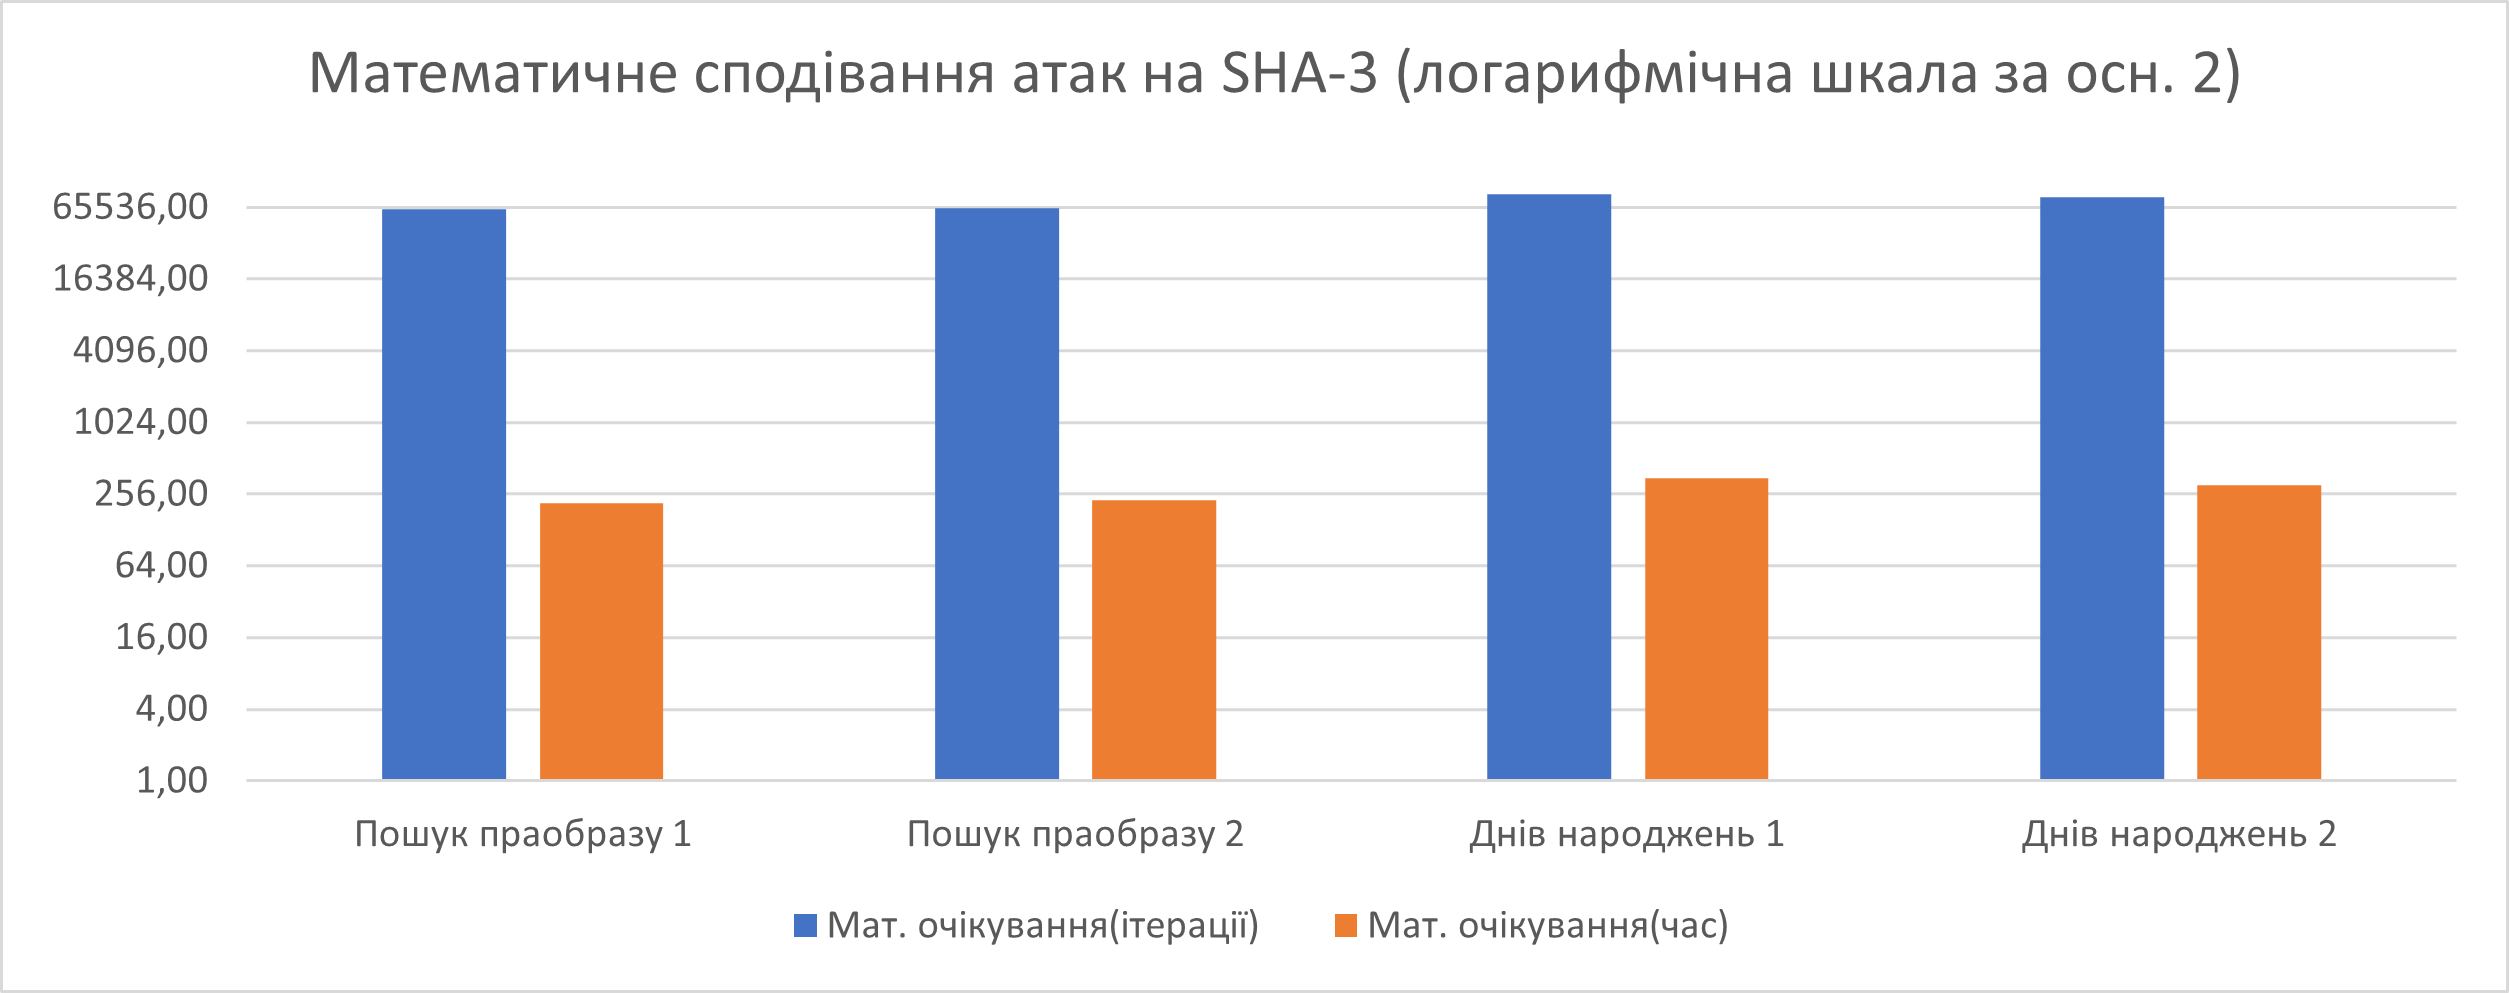
\includegraphics[width=0.75\linewidth]{diagram1.png}
    \caption{Математичне сподівання наведених атак}
    \label{fig:enter-label1}
\end{figure}

\begin{figure}[H]
    \centering
    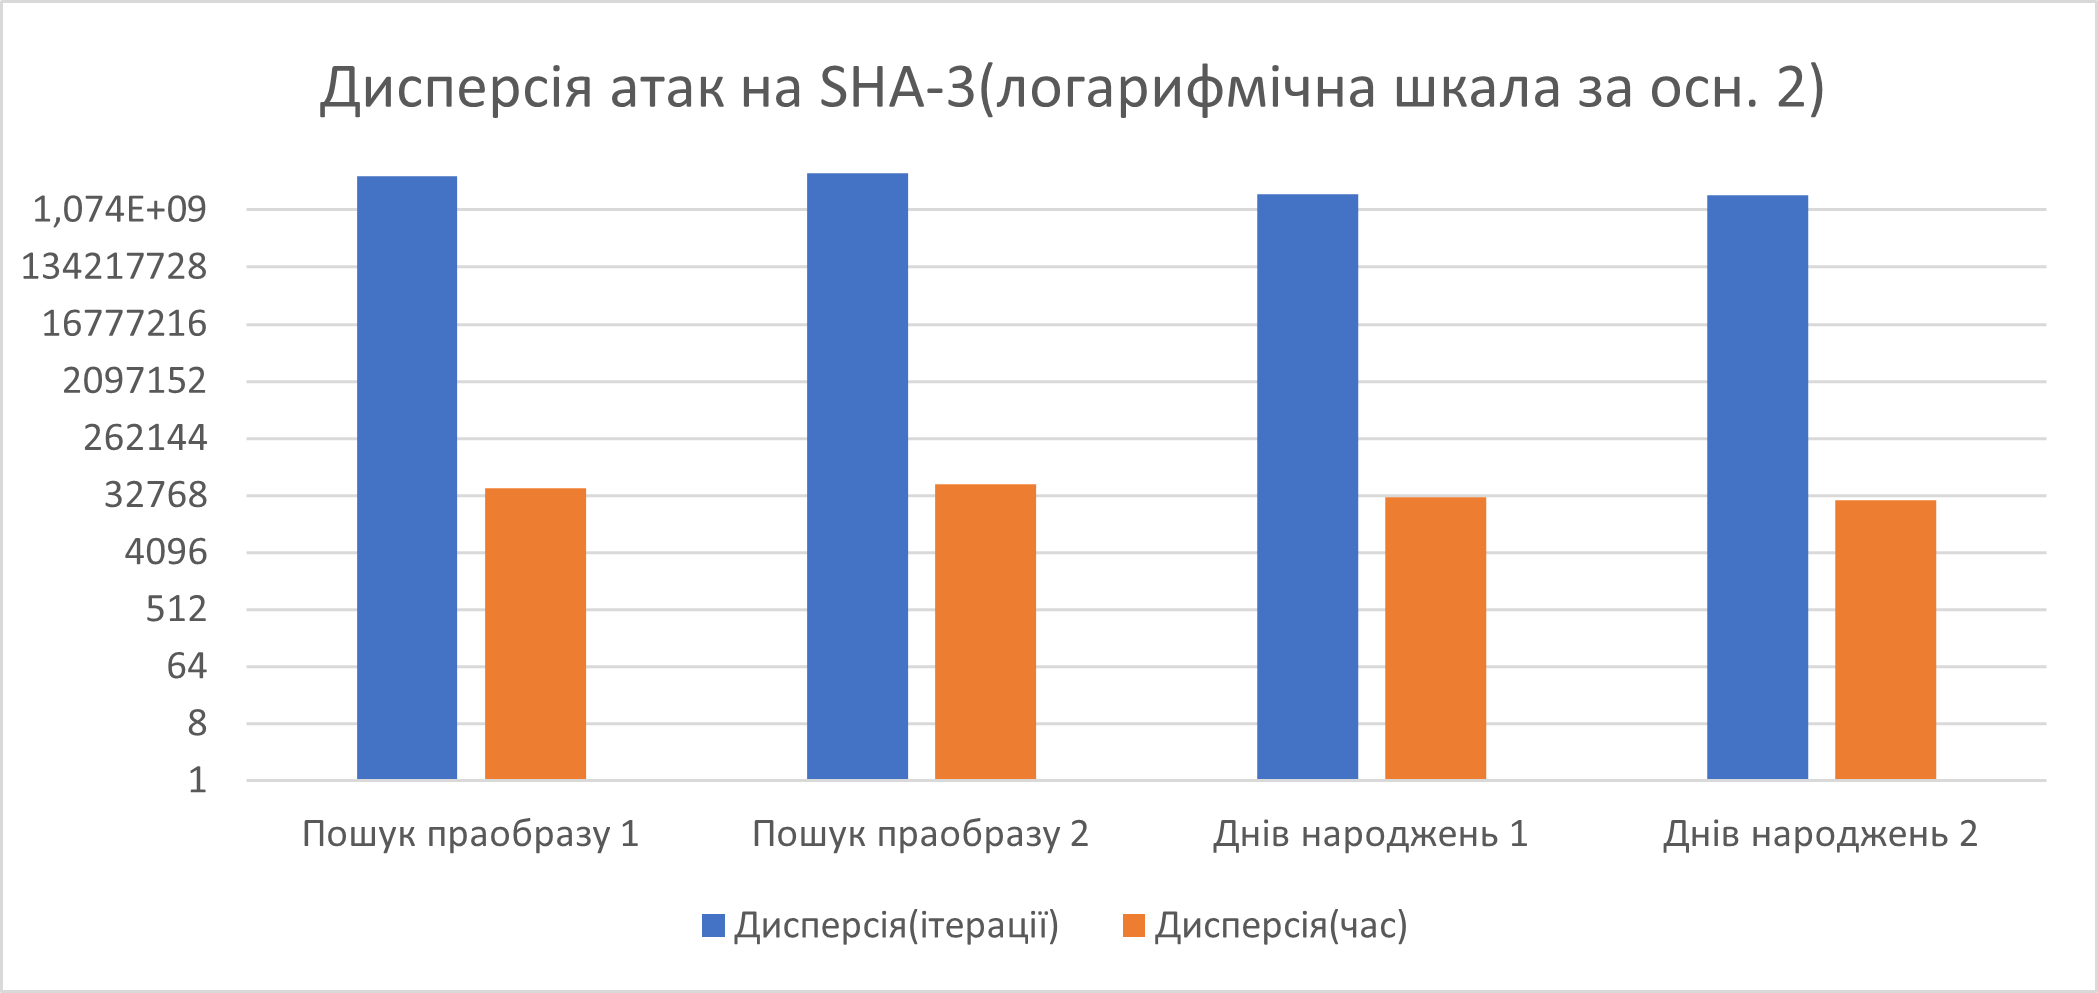
\includegraphics[width=0.75\linewidth]{diagram2.png}
    \caption{Дисперсія наведених атак}
    \label{fig:enter-label2}
\end{figure}

\section{Висновки}

Як видно з графіків та таблиць, в моїй реалізації не так суттєво відрізняються атаки пошуку праобразу та днів народжень, хоча в середньмоу, атака днів народжень має більше математичне сподівання, але меншу дисперсію, і, відповідно, стандартне відхилення. 

Теоритична складність атаки пошуку праобразу на SHA-3-224: $O(2^c = 2^{2n} = 2^{448})$.
На урізану версію до 16 бітів- $2^16$, що потрапляє в наш довірчий інтервал для двох стратегій. З іншого боку, атака послідовного додавання числа виявилась трохи ефективнішою, хоча, насправді, несуттєво відрізняється.

Теоритична складність пошуку колізії для SHA-3-224: $O(2^{\frac{c}{2}}) = 2^n = 2^{224}$. На урізану версію SHA-3-224 до 32 бітів теоритично, має були склданість $2^16$. Але практичні результати виявились трохи більшими.

\section{Додаток А: Результати атак}

\subsection{Атака пошуку праобразу}

\textbf{Стратегія додавання числа до повідомлення}

\noindent
Початкове повідомлення: IsachenkoNikitaSergiyovich57371.

\noindent
Перші 30 згенерованих повідомлень:
\begin{verbatim}
IsachenkoNikitaSergiyovich573710
IsachenkoNikitaSergiyovich573711
IsachenkoNikitaSergiyovich573712
IsachenkoNikitaSergiyovich573713
IsachenkoNikitaSergiyovich573714
IsachenkoNikitaSergiyovich573715
IsachenkoNikitaSergiyovich573716
IsachenkoNikitaSergiyovich573717
IsachenkoNikitaSergiyovich573718
IsachenkoNikitaSergiyovich573719
IsachenkoNikitaSergiyovich5737110
IsachenkoNikitaSergiyovich5737111
IsachenkoNikitaSergiyovich5737112
IsachenkoNikitaSergiyovich5737113
IsachenkoNikitaSergiyovich5737114
IsachenkoNikitaSergiyovich5737115
IsachenkoNikitaSergiyovich5737116
IsachenkoNikitaSergiyovich5737117
IsachenkoNikitaSergiyovich5737118
IsachenkoNikitaSergiyovich5737119
IsachenkoNikitaSergiyovich5737120
IsachenkoNikitaSergiyovich5737121
IsachenkoNikitaSergiyovich5737122
IsachenkoNikitaSergiyovich5737123
IsachenkoNikitaSergiyovich5737124
IsachenkoNikitaSergiyovich5737125
IsachenkoNikitaSergiyovich5737126
IsachenkoNikitaSergiyovich5737127
IsachenkoNikitaSergiyovich5737128
IsachenkoNikitaSergiyovich5737129    
\end{verbatim}

Загальна кількість ітерацій $N = 53193$.

Знайдена колізія: (IsachenkoNikitaSergiyovich57371, IsachenkoNikitaSergiyovich5737153192)

\begin{align*}
m_1 &= \text{IsachenkoNikitaSergiyovich57371}; \\
m_2 &= \text{IsachenkoNikitaSergiyovich5737153192}; \\
h(m_1) &= \textcolor{codegray}{\text{9625d914b345eb5171f683a430e0f277f25a16df708b433a828a}}\text{\textbf{d00e}} \\
h(m_2) &= \textcolor{codegray}{\text{676855f7fc1ade01a82486edc5738d97a56e0e45dc7462bcf3d0}}\text{\textbf{d00e}}
\end{align*}

\subsection{Атака Днів Народжень}

\textbf{Стратегія додавання числа до повідомлення}

\noindent
Початкове повідомлення: IsachenkoNikitaSergiyovich6063

\noindent
Перші 30 повідомлень:
\begin{verbatim}
IsachenkoNikitaSergiyovich60630
IsachenkoNikitaSergiyovich60631
IsachenkoNikitaSergiyovich60632
IsachenkoNikitaSergiyovich60633
IsachenkoNikitaSergiyovich60634
IsachenkoNikitaSergiyovich60635
IsachenkoNikitaSergiyovich60636
IsachenkoNikitaSergiyovich60637
IsachenkoNikitaSergiyovich60638
IsachenkoNikitaSergiyovich60639
IsachenkoNikitaSergiyovich606310
IsachenkoNikitaSergiyovich606311
IsachenkoNikitaSergiyovich606312
IsachenkoNikitaSergiyovich606313
IsachenkoNikitaSergiyovich606314
IsachenkoNikitaSergiyovich606315
IsachenkoNikitaSergiyovich606316
IsachenkoNikitaSergiyovich606317
IsachenkoNikitaSergiyovich606318
IsachenkoNikitaSergiyovich606319
IsachenkoNikitaSergiyovich606320
IsachenkoNikitaSergiyovich606321
IsachenkoNikitaSergiyovich606322
IsachenkoNikitaSergiyovich606323
IsachenkoNikitaSergiyovich606324
IsachenkoNikitaSergiyovich606325
IsachenkoNikitaSergiyovich606326
IsachenkoNikitaSergiyovich606327
IsachenkoNikitaSergiyovich606328
IsachenkoNikitaSergiyovich606329
\end{verbatim}

Загальна кількість ітерацій $N = 134048$.

Знайдена колізія:

(IsachenkoNikitaSergiyovich6063134047, IsachenkoNikitaSergiyovich606350021)

\begin{align*}
m_1 &= \text{IsachenkoNikitaSergiyovich6063134047}; \\
m_2 &= \text{IsachenkoNikitaSergiyovich606350021}; \\
h(m_1) &= \textcolor{codegray}{\text{a3705dfd0fc011cf5612c2715266d55f2a4c7db1960f9015}}\text{\textbf{1c4c4599}} \\
h(m_2) &= \textcolor{codegray}{\text{53cd527720c372f375763e8cefdf3e1af608e01b19d88154}}\text{\textbf{1c4c4599}}
\end{align*}

\textbf{Стратегія випадкової зміни повідомлення}

\noindentПочаткове повідомлення: IsachenkoNikitaSergiyovich36950;

\noindent Перші 30 згенерованих\footnote{Оскільки заміна відбувається на довільний ASCII символ, можуть трапитись спеціальні символи, які впливають на відображення інших символів. Тому тут і далі наводяться значення в спеціальній формі, але при спробі взяти геш від них-- отримаємо зовсім інший геш} повідомлень:
\begin{verbatim}
IsachenkoNikitaSergiyovich36,50
IsachenkoNikitaSergiy<vich36,50
Isachenko$ikitaSergiy<vich36,50
Isachenko$ikitaSeCgiy<vich36,50
Isachenko$ikitaSeCgiy<vich36,\u{1c}0
Isachenko$ikitaSeCgiy<v\u{c}ch36,\u{1c}0
Isachenko$ikitaSeCgiy<v\u{c}ch36,\u{1c}K
Isachenko$ikitaSe0giy<v\u{c}ch36,\u{1c}K
Isachenk\u{13}$ikitaSe0giy<v\u{c}ch36,\u{1c}K
Isachenk\u{13}$iXitaSe0giy<v\u{c}ch36,\u{1c}K
Isachenk\u{13}$iXitaSe0gCy<v\u{c}ch36,\u{1c}K
Isachenk\u{13}$iXitaSe\u{1a}gCy<v\u{c}ch36,\u{1c}K
Isachenk\u{13}$iXitaSe\u{1a}gCy<v\u{c}ch36?\u{1c}K
Isachenk\u{13}$iXit?Se\u{1a}gCy<v\u{c}ch36?\u{1c}K
Isachenk{$iXit?Se\u{1a}gCy<v\u{c}ch36?\u{1c}K
Isachenk{$iXit?Se\u{1a}gCy<v\u{c}ch34?\u{1c}K
ISachenk{$iXit?Se\u{1a}gCy<v\u{c}ch34?\u{1c}K
ISachenk{$iXit?Se\u{1a}gCy<v\u{c}ch34?qK
ISachenk{$iLit?Se\u{1a}gCy<v\u{c}ch34?qK
ISachenk{$iLit?Se\u{1a}gCy\0v\u{c}ch34?qK
ISachenk{$iLYt?Se\u{1a}gCy\0v\u{c}ch34?qK
nSachenk{$iLYt?Se\u{1a}gCy\0v\u{c}ch34?qK
nSachynk{$iLYt?Se\u{1a}gCy\0v\u{c}ch34?qK
nSachynk{$iLYt?Se\u{1a}gCz\0v\u{c}ch34?qK
nSachynk{$iLYtKSe\u{1a}gCz\0v\u{c}ch34?qK
nSachynk{$iLYtKSe\u{1a}gCz\0v\u{c}vh34?qK
nSachynk{$iLYtKSe\u{1a}gCz\0v\u{c}vh346qK
nSachynk{$iLYtKSe\u{1a}gCz\0v\u{c}vh=46qK
nSachynk{$iLYtKSe\u{1a}gCz\0v\u{c}vh=4UqK
nSachynk{$iLYtKSe\u{1a}gCz\\v\u{c}vh=4UqK
\end{verbatim}

\noindentКількість ітерацій: 54193.

Знайдена колізія: 
\begin{verbatim}
    (yWOR\\\u{1}W|c8Q\r\u{19}\u{1a}-=c\u{1b}\u{15}h]
    {\u{2}\u{4}=E\u{1c}\u{6}\u{13}'\u{11},
    3\u{12} R!q\u{1b}@Xe/\"+fu>\\\u{7f}KO\u{11}l`\u{e}ijS2{\u{1f}/)
\end{verbatim}

\begin{align*}
h(m_1) &= \textcolor{codegray}{\text{71c28c19a74a102877417609974d6a2fc9ec4cd174398419}}\text{\textbf{fa2e1868}} \\
h(m_2) &= \textcolor{codegray}{\text{ec4b1a6e9fcf1c04da59b3281f03ae43b20197da6c63c0f2}}\text{\textbf{fa2e1868}}
\end{align*}

\section{Додаток Б: Сирцевий код стратегій модифікації повідомлень та атак}

Реалізація стратегій модифікації рядків:
\begin{lstlisting}[language=rust]
    impl<'a> StringModificator<'a> for AdditionStringModifier<'a> {
    fn modify(&mut self) -> String {
        let mut res = String::from(self.data);
        res.push_str(&self.state.get().to_string());
        self.state.set(self.state.get() + 1);
        res
    }
    ...
    }

    impl<'a> StringModificator<'a> for RandomChangeStringModifier {
    fn modify(&mut self) -> String {
        let mut changable_str = self.data.clone().into_bytes();
        let mut rng = thread_rng();
        let random_pos:usize = rng.gen_range(0..self.data.len());
        loop {
            let random_change:u8 = rng.gen_range(0..128); // because we want ascii in utf8
            if random_change != changable_str[random_pos as usize] {
                changable_str[random_pos as usize] = random_change;
                break;
            }
        }
        match String::from_utf8(changable_str) {
            Ok(val) => {
                self.data = val.clone();
                val
            },
            _ => String::new()
        }
    }
    ...
    }
\end{lstlisting}

Атаки пошуку праобразу, та днів народжень:

\begin{lstlisting}
fn second_preimage_attack<'a, T>(s: &'a str) -> AttackResult
where
T: StringModificator<'a>
{
    let hashed_value = hash(s);
    let mut modifier: T = T::from_str(s);
    let mut iter_count: u64 = 0;
    loop {
        iter_count += 1;
        let modified_value = modifier.modify();
        let hashed_modified_value = hash(&modified_value);
        if &hashed_value[hashed_value.len() - 4..] == &hashed_modified_value[hashed_modified_value.len() - 4..] {
            return AttackResult {
                iterations_count: iter_count,
                collision : (s.to_owned(), modified_value)
            };
        }
    }
}

fn birthday_attack<'a, T>(s: &'a str) -> AttackResult
where
T : StringModificator<'a>
{
    let mut hash_set = HashMap::<String, String>::new();
    let mut modifier: T = T::from_str(s);
    let mut iter_count: u64 = 0;
    loop {
        let val = modifier.modify();
        let hash_val = hash(&val);
        let hash_val = &hash_val[hash_val.len() - 8..];
        iter_count += 1;
        if let Some(finded) = hash_set.get(hash_val) {
            return AttackResult {
                iterations_count: iter_count,
                collision: (val, finded.to_owned())
            };
        } else {
            hash_set.insert(hash_val.to_owned(), val);
        }
    }
}
\end{lstlisting}


\end{document}
